% vim: set spelllang=fr foldmethod=marker:
\section{Mise en place de la détection des attaques}
\label{sa:sec:detection}
%===============================================================================
    \subsection{Hypothèses de travail}\label{sa:ssec:hypotheses}

Sauf indication contraire, les travaux exposés dans le présent chapitre, ainsi par ailleurs que dans les chapitres~\ref{chap:se} et~\ref{chap:sd}, reposent sur les hypothèses suivantes:
\begin{itemize}
    \item Le contexte est celui d'un \rcsf constitué de nœuds possédant tous les mêmes caractéristiques physiques et techniques et limités en ressources disponibles, ainsi que d'une \sdb «non limitée» en ressources.
    \item Pour en faciliter la gestion, ce réseau est partitionné en clusters. Les mécanismes déployés au sein de chaque cluster sont identiques, si bien qu'il est possible, pour les décrire, de ne traiter que le cas d'un seul cluster.
    \item Au sein des clusters toujours, tous les capteurs peuvent atteindre le \ch en un seul saut: ils n'ont donc pas besoin de moduler la puissance de leurs transmissions. Les \chs sont les seuls à recourir à cette possibilité pour atteindre directement la \sdb, si aucun protocole de \idx{routage} inter-clusters n'a été mis en place.
    \item La \idx{mobilité} des nœuds est faible, voir nulle; elle est en tout cas négligeable par rapport à l'échelle temporelle utilisée dans les protocoles mis en place, et les nœuds sont donc considérés comme statiques.
    \item Le but final recherché est la détection d'un attaquant qui mènerait un assaut contre le réseau en introduisant ou en compromettant un capteur (il s'agit donc d'un attaquant interne, équipé d'un matériel de caractéristiques identiques aux autres capteurs).
\end{itemize}

%===============================================================================
    \subsection{Objectifs à atteindre}

Le but de la solution proposée est de fournir un moyen efficace de détecter un nœud compromis dans le réseau, qui tenterait par exemple de saturer les capacités de communication du réseau, en envoyant un flux de données plus important que les nœuds «honnêtes».
Plusieurs attaques peuvent être détectées par l'application de règles sur le trafic qui transite au sein du réseau (voir le paragraphe correspondant au \chapref{ea}, \ssref{ea:par:rules}).
Le modèle qui vient d'être donné sera celui repris à titre d'exemple tout au long de la description de la méthode.

Dans ce contexte, le modèle de l'attaque étudié est donc le suivant: un capteur compromis, sous la direction de l'attaquant, transmet un volume de données (que ce soit par la taille ou bien par le nombre de paquets envoyés) bien plus élevé que ce qu'il devrait, ce qui peut mener:
\begin{itemize}
    \item à l'accaparement\index{comportement cupide!accaparement} du canal de transmission, ce qui peut empêcher les nœuds légitimes d'envoyer leurs propres messages;
    \item à des congestions\index{congestion} sur le trafic, par exemple si les paquets sont envoyés à un rythme trop soutenu pour que le \CH ait le temps de tous les traiter;
    \item à l'épuisement des nœuds en écoute, et notamment du \ch submergé de données à retransmettre;
    \item à l'altération de la représentativité des données obtenues par l'exploitant, surtout dans le cas où les paquets contiennent des données erronées.
\end{itemize}

L'efficacité d'une méthode de détection de ce nœud compromis peut être mesurée sur deux aspects:
\begin{itemize}
    \item le taux de détection du ou des nœud(s) compromis dans le réseau;
    \item la durée de vie du réseau.
\end{itemize}
Le second critère peut lui-même être exprimé de plusieurs façons.
Par exemple, il peut être directement associé à la durée de vie du dernier capteur restant dans le réseau; mais ce capteur seul n'est plus forcément à même de fournir un service efficace.
Aussi la durée de vie du réseau est-elle souvent définie comme la durée écoulée entre le déploiement du réseau et l'instant où le premier capteur à manquer d'énergie s'éteint.
C'est cette deuxième définition qui sera utilisée par la suite.
Elle implique que pour obtenir une grande durée de vie, la consommation en énergie du réseau doit être équitablement répartie entre un aussi grand nombre de nœuds que possible.

Pour obtenir une méthode efficace sur les deux points évoqués, nous proposons dès lors d'accompagner la mise en place des nœuds de surveillance par deux mécanismes: une partition hiérarchique récursive\index{clusterisation!partition récursive} des nœuds du réseau d'une part, et une sélection dynamique\index{selection@sélection!sélection dynamique} des «sentinelles» d'autre part.

%===============================================================================
    \subsection{Partition hiérarchique\index{clusterisation!clusterisation hiérarchique} du réseau}

Le fait de clusteriser le \rc tel que présenté au \chapref{st}, \ssref{st:subsec:partition} permet de limiter la consommation en énergie de la plupart des nœuds du réseau, puisque seuls les \chs se retrouvent à effectuer des émissions sur des distances plus longues que le rayon d'un cluster.
La partition récursive\index{clusterisation!partition récursive} permet d'obtenir une gestion encore plus efficace des clusters, puisqu'elle introduit plus de granularité.
Nous proposons, pour notre solution (et pour nos tests, voir \sref{sa:sec:resultats}), une hiérarchie à deux degrés: nous avons clusterisé notre réseau en utilisant $k$-\leach, en fixant $k=2$ (voir \figref{sa:fig:network}).
\begin{figure}[ht]
    \centering
    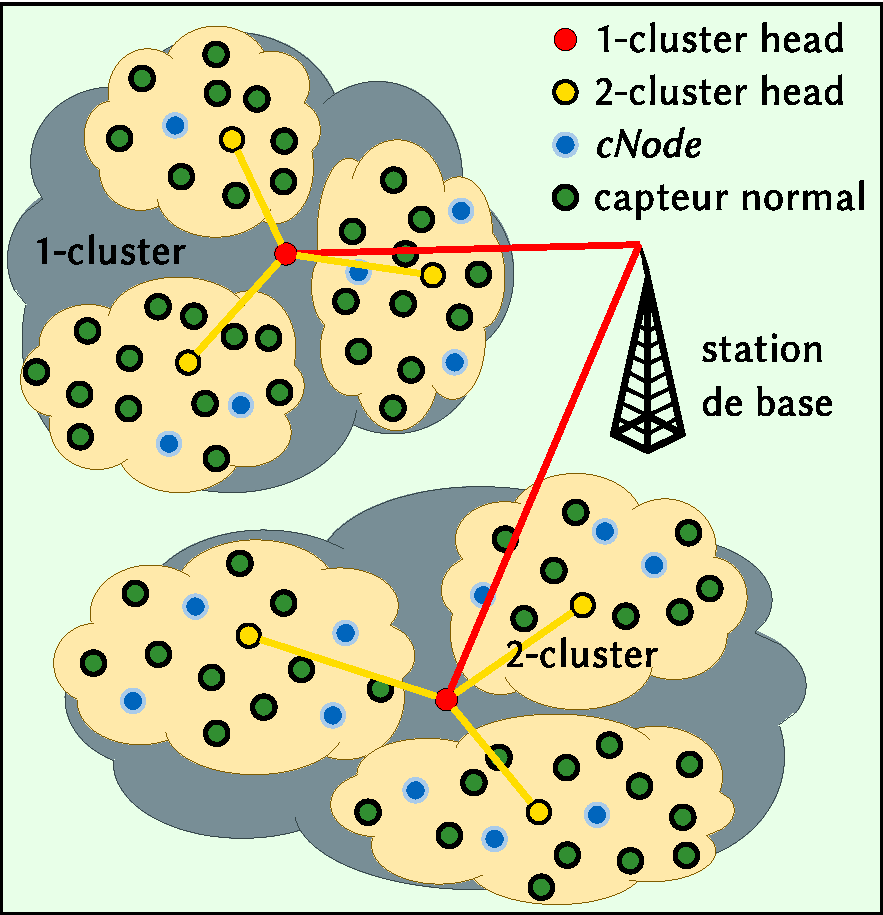
\includegraphics[width=.7\linewidth]{\chapterfig/2-clustered_network.pdf}
    \caption{Schéma du réseau avec deux niveaux de partition}\label{sa:fig:network}
\end{figure}
Ceci permet, à notre sens:
\begin{itemize}
    \item d'économiser davantage d'énergie par rapport à l'usage de \leach dans sa version simple;
    \item d'obtenir, en choisissant des nœuds de surveillance dans chacun des $2$-clusters, une meilleure couverture du réseau par les sentinelles, et de maximiser ainsi la probabilité de détection des nœuds compromis dans le réseau.
\end{itemize}
En pratique, $k$ doit être adapté en fonction du nombre de capteurs dans le réseau, de sa superficie, de la puissance et de la consommation énergétique des nœuds, et même des applications utilisées dans le réseau.
Des expériences ayant recours au matériel considéré sont indispensables pour déterminer les valeurs numériques optimales pour un réseau donné, ce qui empêche de fournir ici une estimation numérique: nous nous en tenons donc au degré $2$.

%===============================================================================
    \subsection{Des \cns pour surveiller le trafic}

La partition hiérarchique\index{clusterisation!clusterisation hiérarchique} d'un réseau en clusters établit déjà une distinction entre deux rôles que peuvent assumer les capteurs: celui de nœud «normal», qui poursuit ses opérations de captage et de retransmission des données de façon classique, et celui de \ch, qui se retrouve chargé d'assurer la liaison entre les membres de son cluster et le restant du réseau.
À côté des nœuds «normaux» et des \chs, un troisième rôle va être attribué à certains capteurs, afin d'assurer la détection des attaques par \dds.
Certains capteurs se voient ainsi confier le rôle de «nœuds de contrôle», ici nommés \cns (introduits sous le nom de \textit{gNodes}\index{gNodes@\textit{gNodes}} dans~\cite{LC08}), et sont chargés de surveiller le trafic entrant et sortant des \chs.

Si un \cn constate qu'un capteur envoie, au cours d'une unité de temps, plus de données à leur \CH qu'une valeur de seuil déterminée $S_{\textrm{débit}}$, il retient que le nœud a eu un comportement anormal (il y a eu un écart important à la moyenne de la quantité de données envoyées par unité de temps).
Lorsque ce nœud réalise un certains nombres d'écarts, \cad lorsque le nombre de comportement anormaux détectés par un \cn dépasse une valeur de seuil $S_{\textrm{écarts}}$, le ou les nœuds de contrôle qui ont repéré ces écarts considèrent alors le capteur comme compromis.
Chaque \cn ayant détecté un nœud compromis envoie un message d'avertissement à son \ch.
Ici encore, un seuil $S_{\textrm{alertes}}$ est fixé pour le nombre minimum d'alertes qu'un \CH doit recevoir avant de considérer un nœud comme malveillant, et ce afin d'éviter qu'un nœud compromis se faisant passer pour un \cn ne déclare tous ses voisins comme compromis.
Plusieurs \cns distincts doivent donc détecter les écarts d'un nœud pour que celui-ci soit effectivement considéré comme compromis par le \ch.

Une fois que la malveillance d'un capteur est effectivement actée par un \ch, la charge incombe à ce dernier de prendre des mesures pour mitiger l'attaque.
En pratique, la solution utilisée ici est simple: tous les messages en provenance des nœuds considérés malveillants par le \ch sont ignorés (le \CH se met immédiatement à les ignorer, et il prévient les capteurs du cluster afin qu'ils puissent en faire autant).

Les \cns comparent également la taille des trafics entrant et sortant du \ch.
En cas d'écarts importants (en tenant compte des éventuels facteurs de \idx{compression} des données et des messages ignorés des nœuds considérés compromis), ils peuvent être amenés à penser que le \ch est lui-même malveillant.
Dans ce cas, l'\election d'un nouveau \CH dans le cluster est déclenchée.

%===============================================================================
    \subsection{Sélection dynamique\index{selection@sélection!sélection dynamique} des \cns}

        \subsubsection{Motivations}
La partition\index{clusterisation} du réseau permet de limiter aux seuls \chs les efforts énergétiques dus aux transmissions longues.
L'inconvénient est que, justement, ces \CH vont épuiser leur batterie beaucoup plus rapidement que s'ils étaient restés des nœuds ordinaires, tirant ainsi le réseau vers une fin de vie précoce.
Les nœuds ne sont pas toujours désignés \CH «à vie»: ainsi \leach renouvelle périodiquement la partition du réseau, choisissant à chaque itération de nouveaux \chs et entrainant la sélection\index{selection@sélection} d'un nouveau lot de \cns.

Mais tous les protocoles de clusterisation\index{clusterisation!protocole de clusterisation} ne prévoient pas nécessairement de \idx{renouvellement} régulier de la partition.
De plus, s'ils n'émettent pas sur de longues distances, les \cns se retrouvent eux aussi à consommer plus d'énergie que les nœuds normaux, puisqu'ils doivent sans cesse rester à l'écoute des transmissions qui les entourent, et analyser le débit de chacun de leurs voisins.
Pour répartir cette nouvelle charge, qui touche davantage de nœuds, nous proposons d'élire également les \cns de façon dynamique, sur une période plus courte que celle, éventuelle, qui correspond à la \idx{clusterisation} du réseau.

Il est vrai que le renouvellement périodique\index{renouvellement!renouvellement périodique} des \cns rajoute des contraintes et augmente le volume des messages de contrôle à échanger dans le réseau.
Pour certaines applications des capteurs, ceci peut représenter un inconvénient que la répartition de la charge ne vient pas contrebalancer; mais de manière générale la préservation des réserves énergétiques est primordiale dans les \rcs, et un meilleur équilibre de la charge obtenu pour un prix relativement modeste ne semble pas superflu.
Autre remarque: en matière de détection d'intrusion, les \IDS les plus récents se vantent souvent de n'engendrer qu'un faible surplus de consommation dans le réseau~\cite{LZYP08}, et la question se pose donc de savoir si la répartition de la charge par un renouvellement dynamique\index{renouvellement!renouvellement dynamique} reste pertinente; nous verrons en section suivante qu'avec un système aussi simple que nos \cns, les simulations annoncent un gain important sur la répartition de la charge.
Il faut également garder à l'esprit que les mécanismes de renouvellement périodique\index{renouvellement!renouvellement périodique} et de sélection\index{selection@sélection} des nœuds de surveillance ne sont pas dépendants du mécanisme de détection utilisé (\cad des \cns qui appliquent des règles sur le trafic analysé).
Ainsi, si un \IDS «concurrent»
\begin{itemize}
    \item présente une bonne capacité à économiser l'énergie du réseau,
    \item s'exécute seulement sur un sous-ensemble des nœuds du réseau,
    \item et ne nécessite pas, pour fonctionner, d'équipement distinct du matériel de base des capteurs,
\end{itemize}
alors la dynamique et les méthodes de sélection\index{selection@sélection} présentées dans cette thèse peuvent très bien être mises en œuvre pour optimiser détection et consommation.

Un dernier point reste à signaler.
Cette solution de renouvellement périodique\index{renouvellement!renouvellement périodique} améliore aussi la \secu du réseau: si un attaquant cherche à compromettre tous les \cns du cluster, pour pouvoir poursuivre son attaque discrètement, le renouvellement dynamique\index{renouvellement!renouvellement dynamique} apporte une parade efficace à l'attaque en complexifiant largement le nombre de cibles à corrompre.

        \subsubsection{Le choix par le hasard}
Le renouvellement périodique\index{renouvellement!renouvellement périodique} des capteurs de surveillance peut être réalisé de plusieurs façons.
Dans ce chapitre, une façon de faire très simple est employée: la sélection\index{selection@sélection} des \cns, pour chaque période, est ---~théoriquement~--- aléatoire.
L'aléatoire est une notion délicate en informatique; nous nous contenterons plutôt d'un algorithme capable de générer des nombres dits «pseudo-aléatoires».
Une façon de procéder, par exemple, est de recourir à un algorithme capable de générer une suite de nombre d'apparence aléatoire, utilisés pour déterminer quels seront les \cns pour la période à venir~\cite{BMM13}.
Cet algorithme se doit de respecter les points suivants:
\begin{itemize}
    \item il doit nécessiter peu de calculs;
    \item sa période doit être grande;
    \item les valeurs générées doivent être indépendantes et distribuées uniformément.
\end{itemize}
Nous nous sommes tournés vers un type connu de générateurs, les \textit{Multiplicative Linear-Congruential Generators} (ou MLCG), qui possèdent effectivement une grande période~\cite{RJ91}.
\nomenclature{MLCG}{\textit{Multiplicative Linear-Congruential Generators}}
Plus précisément, le générateur retenu est de type $x_n = a\cdot x_{n-1}\bmod\ m$, où:
\begin{itemize}
    \item le nombre pseudo-aléatoire $x_n$ est généré à partir de son prédécesseur $x_{n-1}$;
    \item $m$ est de la forme $2^k$, ce qui facilite le calcul de $\bmod\ m$ (troncature à droite du résultat sur $k$ bits);
    \item $a$ doit être de la forme $8\cdot i\pm3$ (avec $i$ un entier positif) pour que le générateur ait la période maximale, égale à $2^{k-2}$;
    \item $x_0$ (la «graine», ou \textit{seed} en anglais) doit être un entier impair (toujours pour avoir la meilleure période).
\end{itemize}
La méthode de \textsc{Schrage}\index{methode de schrage@méthode de \textsc{Schrage}} permet de reformuler le générateur sous une forme qui prévient tout problème de débordement\,\footnote{Un débordement désigne le dépassement, au cours des calculs, de la valeur d'entier maximale gérée par le système, et se traduit par des erreurs de calcul.} lors de l'implémentation~\cite{RJ91}.
Le générateur est alors écrit sous la forme suivante: $a\cdot x\bmod m=g(x)+m\cdot h(x)$, avec:
\[\left\{
    \begin{aligned}
        g(x) & =a\cdot(x\bmod q)-r\cdot(x\mbox{~div~}q)\\
        h(x) & =(x\mbox{~div~}q)-(a\cdot x)\mbox{~div~}m\\
        q    & =m\mbox{~div~}a\\
        r    & =m\bmod a
    \end{aligned}
\right.\]
Voici finalement un exemple de générateur (il s'agit de celui qui a été implémenté pour réaliser les tests présentés en \sref{sa:sec:resultats}):
\[x_n=11\cdot x_{n-1}\bmod2^{16}\]
Sa période est égale à $2^{14}$.
Ce générateur peut alors être utilisé pour calculer des nombres pseudo-aléatoires allant de $0$ à $65535$ qui, ramenés sur le nombre attendu de \cns dans le cluster ou bien comparés à un seuil de probabilité, permettent de déterminer quels vont être les nœuds élus pour la période en cours.
Il convient naturellement d'attribuer une graine différente à chaque nœud du réseau, afin d'éviter que tous les nœuds produisent la même suite de nombres pseudo-aléatoires.
Ceci peut être réalisé en initialisant l'algorithme avec une mesure physique ---~après tout, il s'agit de capteurs!~--- dont la valeur est ramenée à l'entier impair le plus proche.

Mais une question subsiste: quelle va-t-être l'entité chargée d'exécuter cet algorithme et de procéder à l'\election des \cns?
Trois méthodes différentes sont ici proposées: une auto-élection\index{selection@sélection!auto-élection} distribuée, une \election centralisée au niveau des \CH, ou alors une \election centralisée au niveau de la \sdb.
%===============================================================================
    \subsection{Processus de sélection\index{selection@sélection} des \cns}

        \subsubsection{Auto-élection\index{selection@sélection!auto-élection} distribuée}
Une première solution consiste à réutiliser l'algorithme d'auto-désignation\index{selection@sélection!auto-élection} mis en œuvre par \leach, comme présenté sur la \figref{sa:fig:elecself}.
Chaque nœud non \CH choisit un nombre pseudo-aléatoire compris entre 0 et 1.
Si ce nombre est en dessous du pourcentage de \cns désirés dans le réseau (et fixé au moment de l'implémentation par l'utilisateur), ce nœud devient un \cn.
Autrement, il reste un capteur normal.
\begin{figure}[ht]
    \centering
    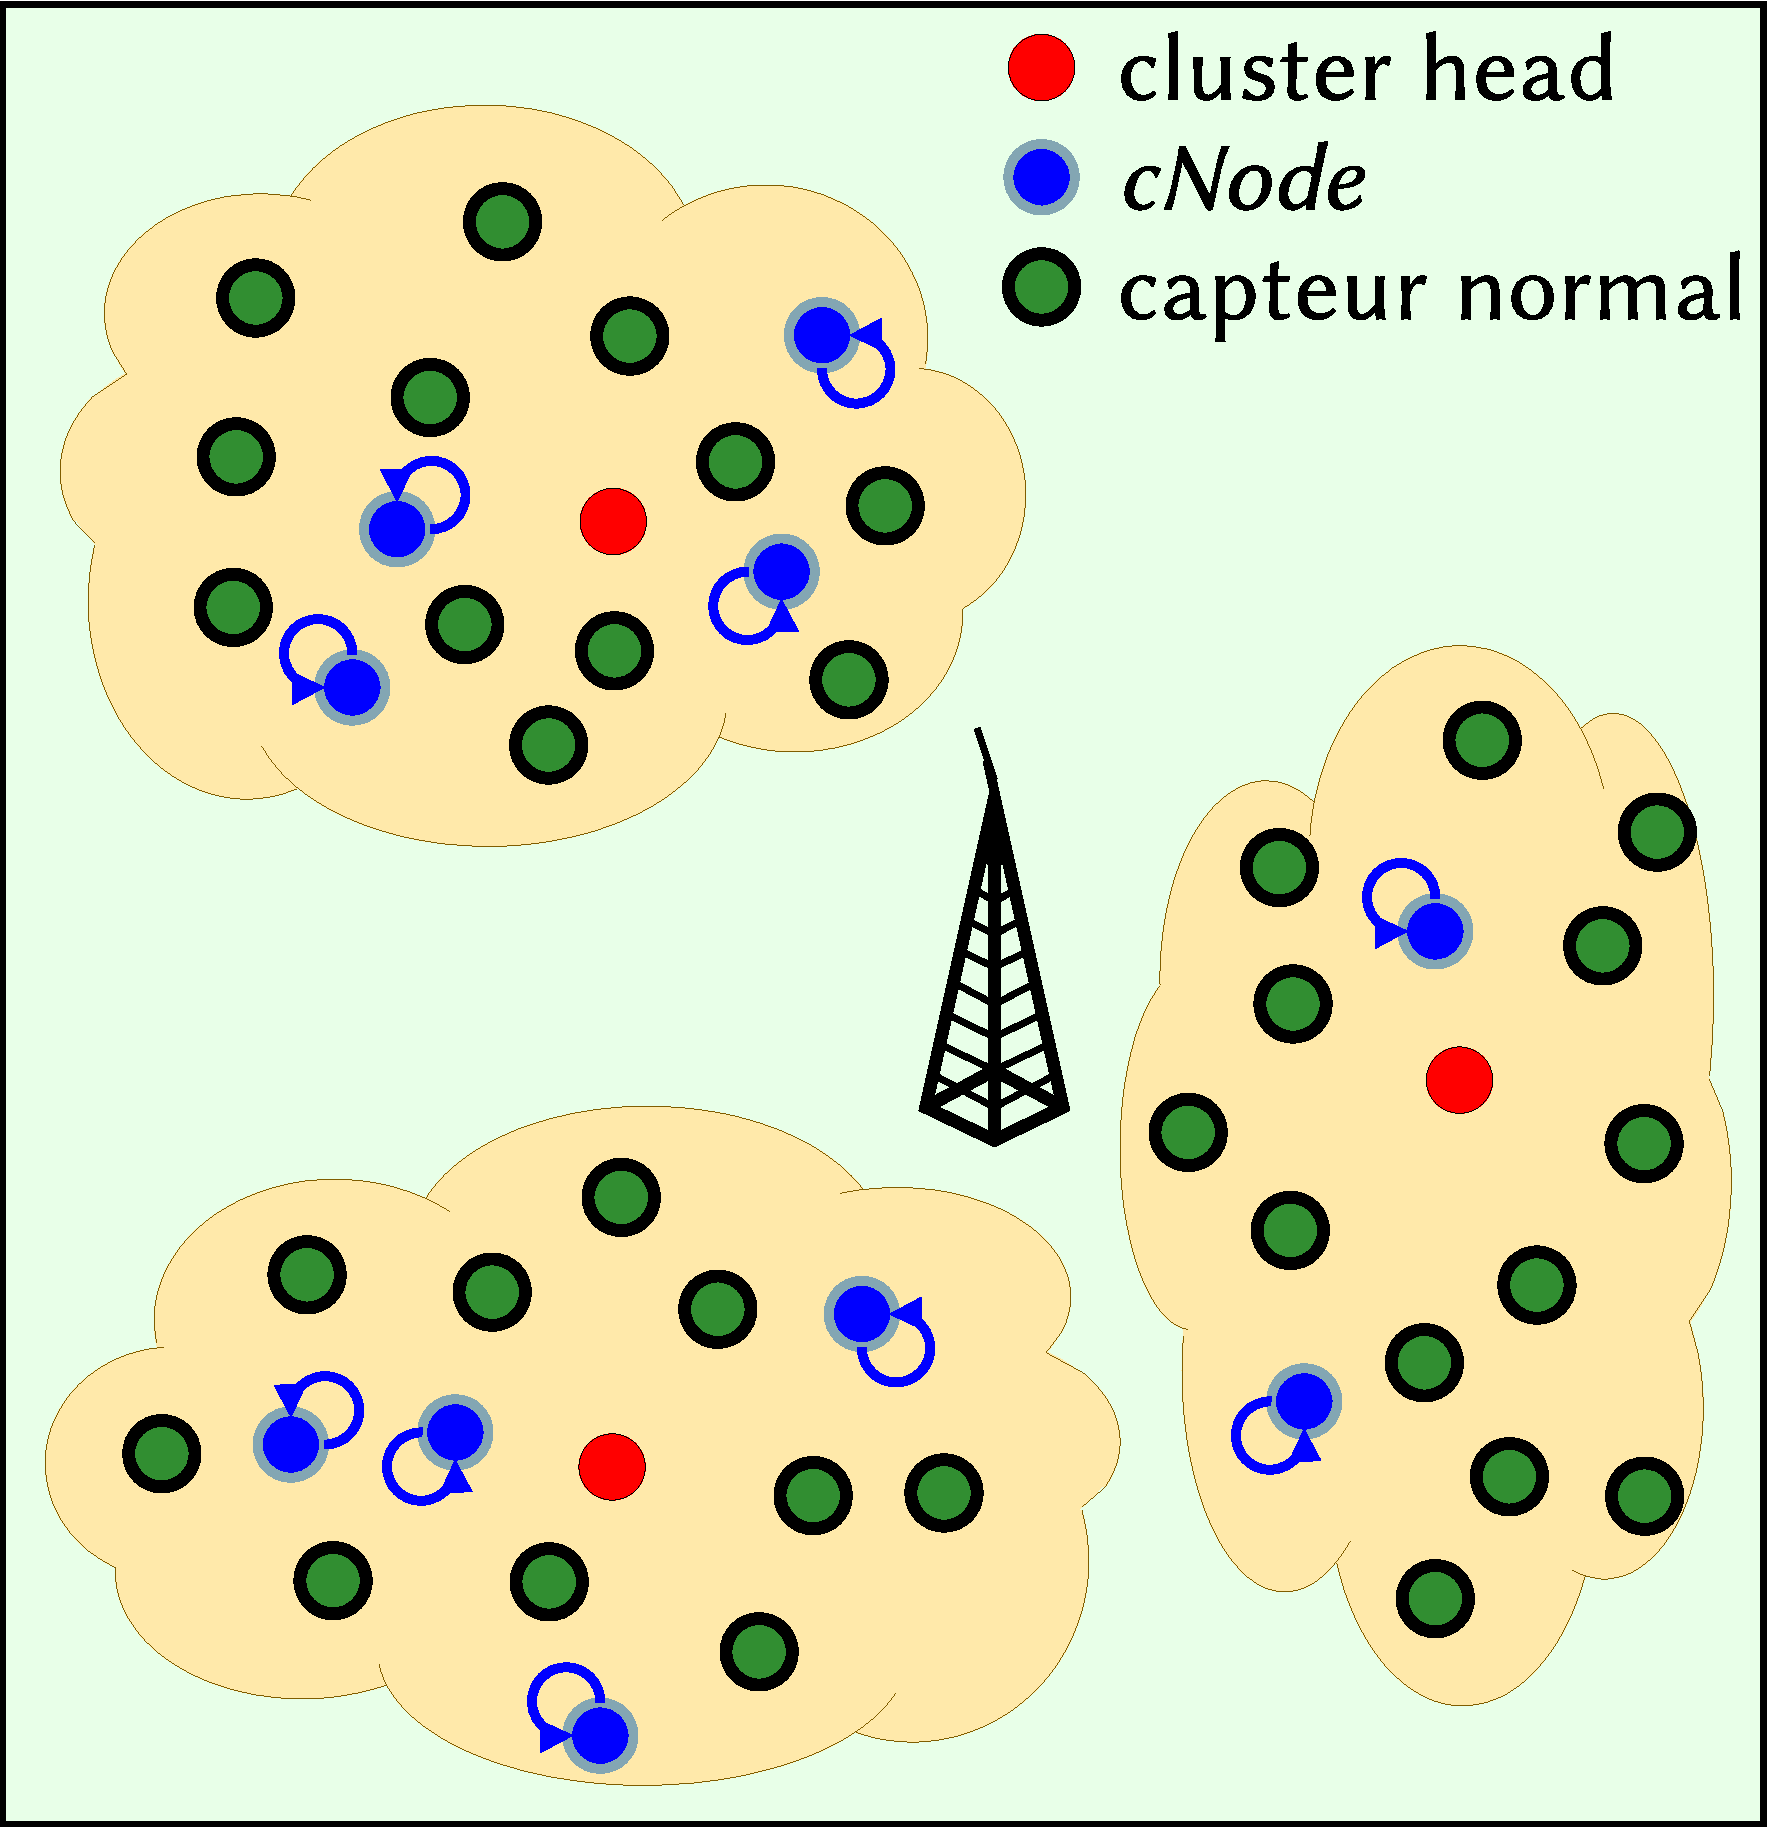
\includegraphics[width=.5\linewidth]{\chapterfig/elec_self.pdf}
    \caption{Auto-élection\index{selection@sélection!auto-élection} des \cns}\label{sa:fig:elecself}
\end{figure}

Cette méthode présente deux inconvénients.
Tout d'abord, elle impose à chaque nœud de calculer un nombre pseudo-aléatoire --- calcul parfois couteux ---, ce qui n'est pas nécessaire avec les deux autres méthodes.
Ensuite, chaque nœud choisit lui-même de se désigner (ou non) \cn, sans tenir compte de la décision de ses voisins.
Si bien que l'\election des \cns ne prend en compte à aucun moment la \idx{clusterisation} du réseau.
Il est très peu probable que les \cns ainsi élus soient uniformément répartis entre les différents $2$-clusters du réseau.
Il est même possible que certains $2$-clusters se retrouvent totalement dépourvus de \cns (et se retrouvent ainsi dans l'incapacité de détecter une attaque).

Ce second point peut être contourné en menant une \election en deux étapes.
Dans un premier temps les nœuds choisissent d'endosser, ou non, le rôle de \cn; les \cns élus signalent alors leur statut au $2$-\CH auquel ils sont associés.
Au cours de la seconde étape, les $2$-\CH nomment des \cns supplémentaires dans leurs $2$-clusters respectifs si le nombre de signalements reçus au regard du nombre de nœuds dans les $2$-clusters est en dessous d'un pourcentage minimal.

        \subsubsection{Élection\index{selection@sélection!election@élection} centralisée au niveau des \chs}
La seconde méthode proposée consiste à décharger les nœuds classiques du processus d'auto-désignation\index{selection@sélection!auto-élection}, pour le remplacer par une nomination autoritaire réalisée par les $2$-\chs (voir \figref{sa:fig:elecch}).
Chaque \CH désigne alors un nombre de \cns correspondant au pourcentage indiqué par l'utilisateur.
Par exemple, si l'on souhaite obtenir dix pour cent de \cns, et qu'un $2$-cluster comporte cent capteurs, le \CH de ce cluster va produire dix nombres pseudo-aléatoires distincts qui seront associés aux identifiants de dix nœuds du cluster.
Le \CH envoie alors un message à chacun de ces dix nœuds pour leur ordonner de remplir le rôle de \cn sur la période en cours.
\begin{figure}[ht]
    \centering
    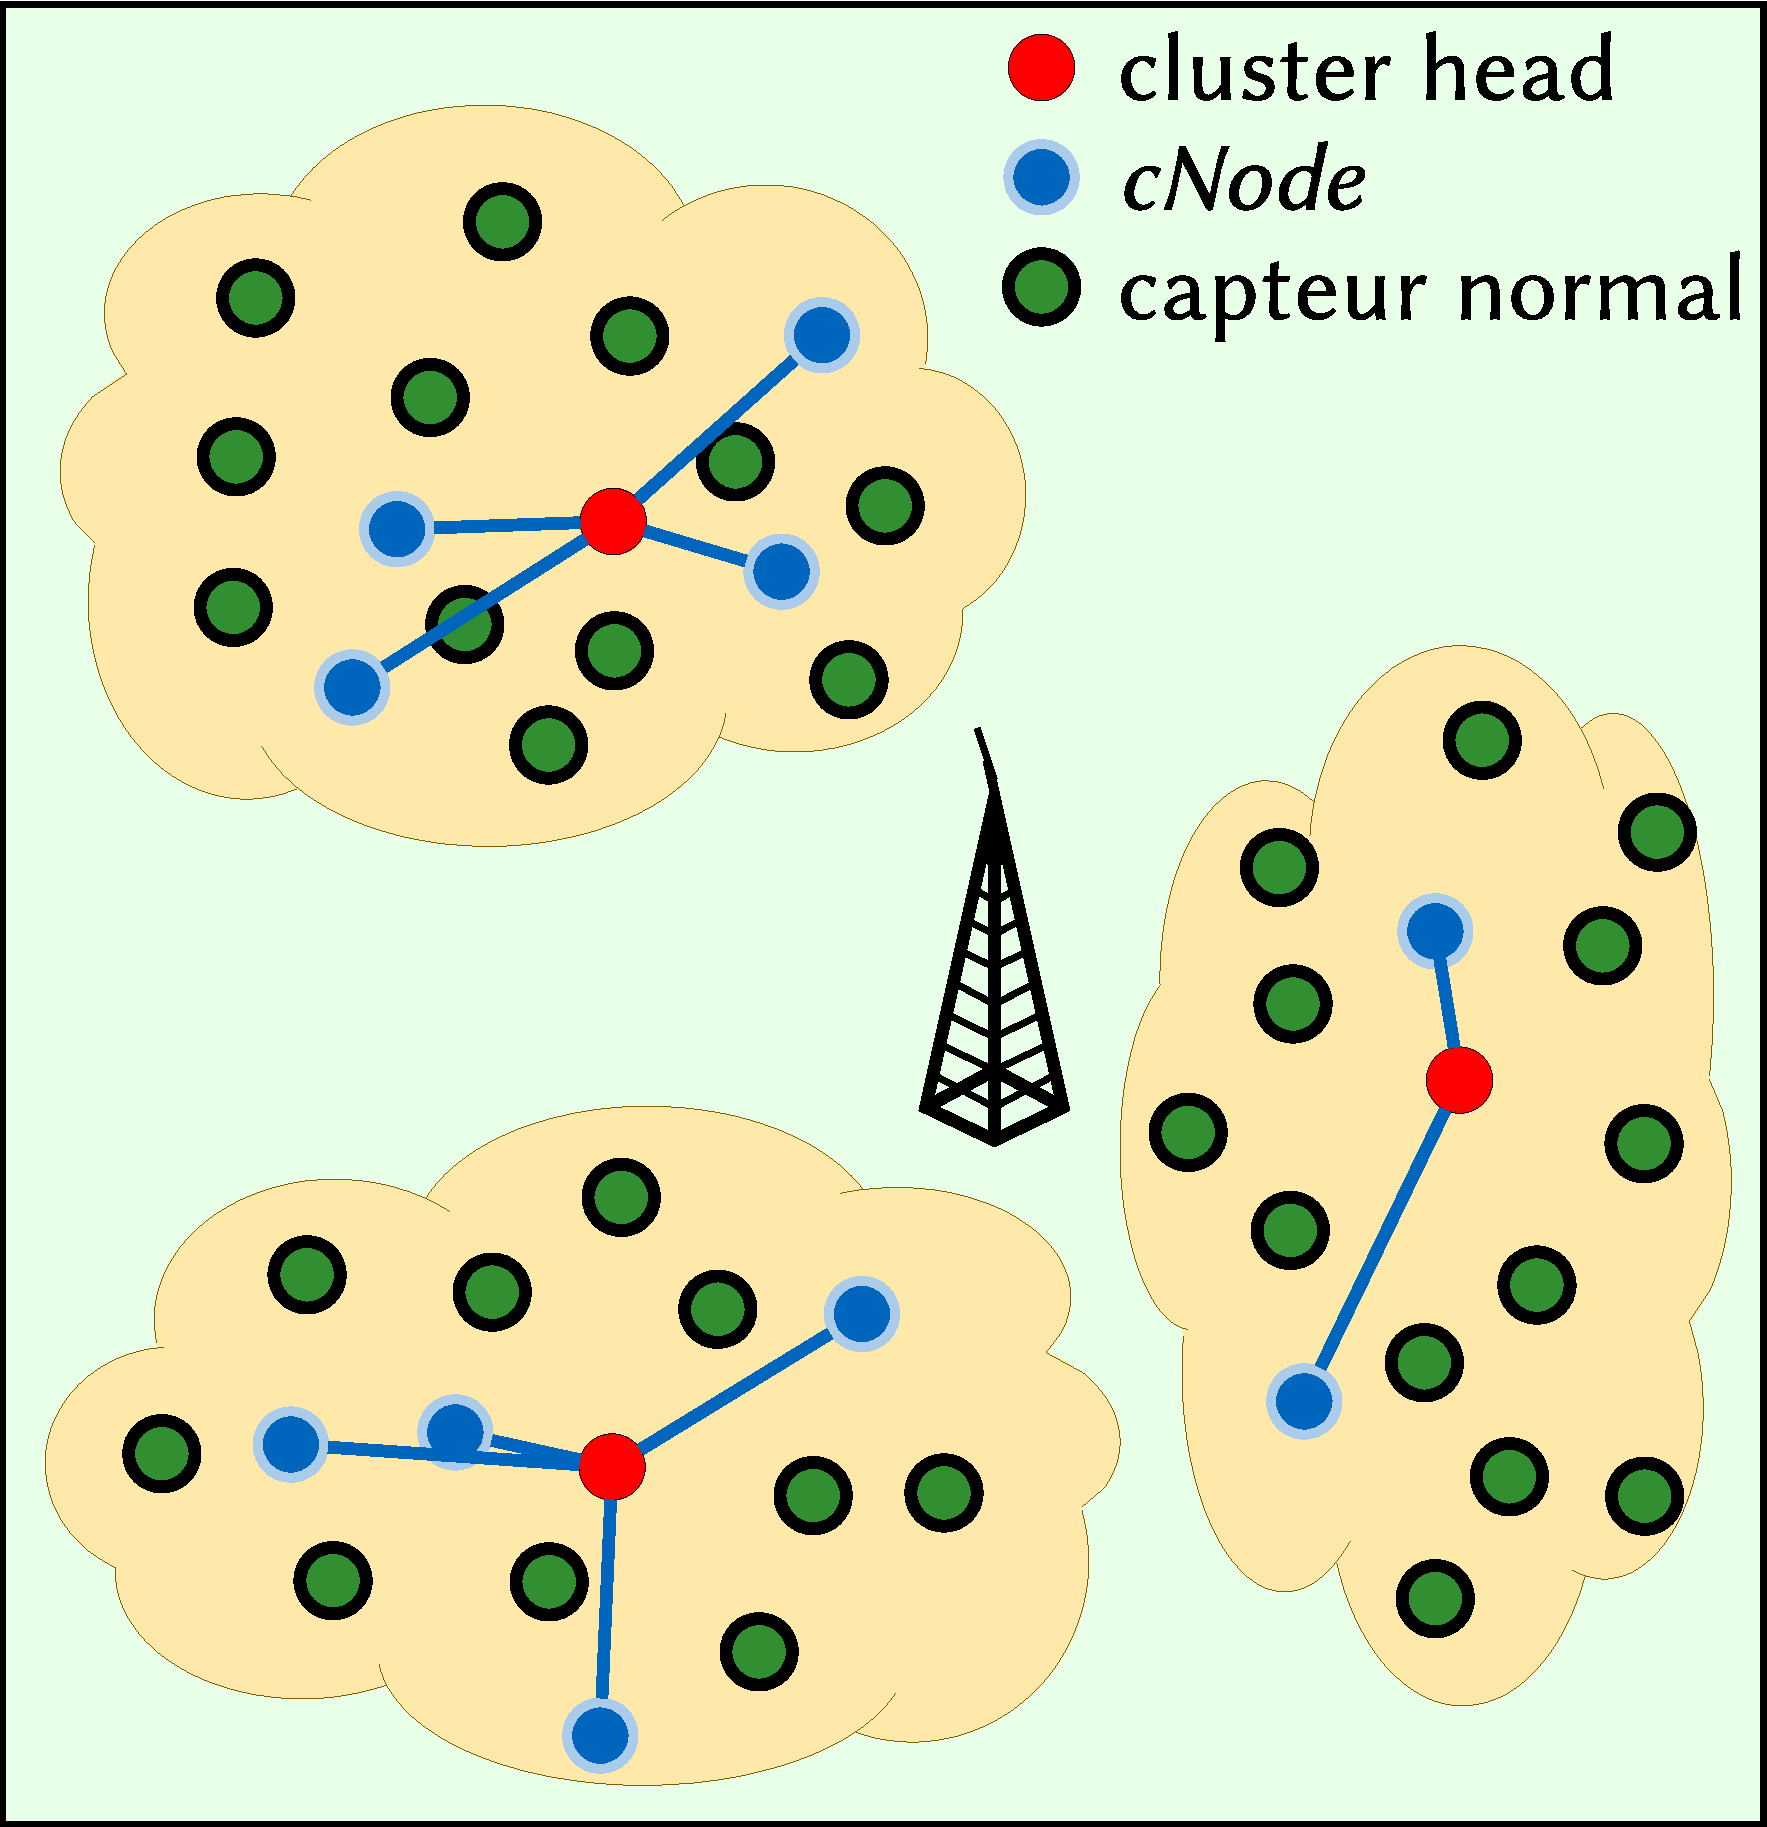
\includegraphics[width=.5\linewidth]{\chapterfig/elec_ch.pdf}
    \caption{Élection\index{selection@sélection!election@élection} des \cns réalisée par les \chs}\label{sa:fig:elecch}
\end{figure}

Cette méthode est plus efficace en ce qui concerne les calculs puisque seuls les $2$-\CH ont à appliquer un algorithme de calcul de nombres pseudo-aléatoires.
Cependant, elle présente un autre désavantage: si l'un de ces \CH est compromis par un attaquant, il ne déclarera sans doute aucun \cn susceptible de le détecter, laissant ainsi tout son cluster à la merci d'autres attaques.
Comme l'algorithme \leach désigne à tour de rôle chaque capteur, sur un cycle complet, pour accomplir le rôle de \CH, tout nœud compromis deviendra logiquement \CH à un moment ou l'autre.
Le problème du \CH ne désignant aucun \cn peut donc légitimement se poser pour n'importe quel nœud compromis du réseau.
Qui plus est, il faut garder à l'esprit que rien n'empêche un nœud compromis de se déclarer \ch à chaque ronde de l'algorithme \leach.

Cette méthode est néanmoins celle qui est implémentée dans les travaux de la référence~\cite{GMT12}, et que nous reprenons pour nos tests (dont les résultats sont disponibles en \sref{sa:sec:resultats}).

        \subsubsection{Élection\index{selection@sélection!election@élection} centralisée au niveau de la \sdb}
L'\election centralisée peut également être effectuée au niveau de la \sdb, comme représenté sur la \figref{sa:fig:elecbs}.
Les $2$-\CH du réseau font alors remonter à la \sdb la liste des nœuds de leurs $2$-clusters respectifs, et celle-ci retourne une liste de \cns pour chacun d'entre eux.
Les capacités (en mémoire, calcul, énergie) de la \sdb étant considérées comme illimitées, cette méthode a pour avantage de déporter toutes les tâches couteuses dans un environnement «sans contraintes».
Le calcul des nombres pseudo-aléatoires par la \sdb ne lui coute, pour ainsi dire, rien.
\begin{figure}[ht]
    \centering
    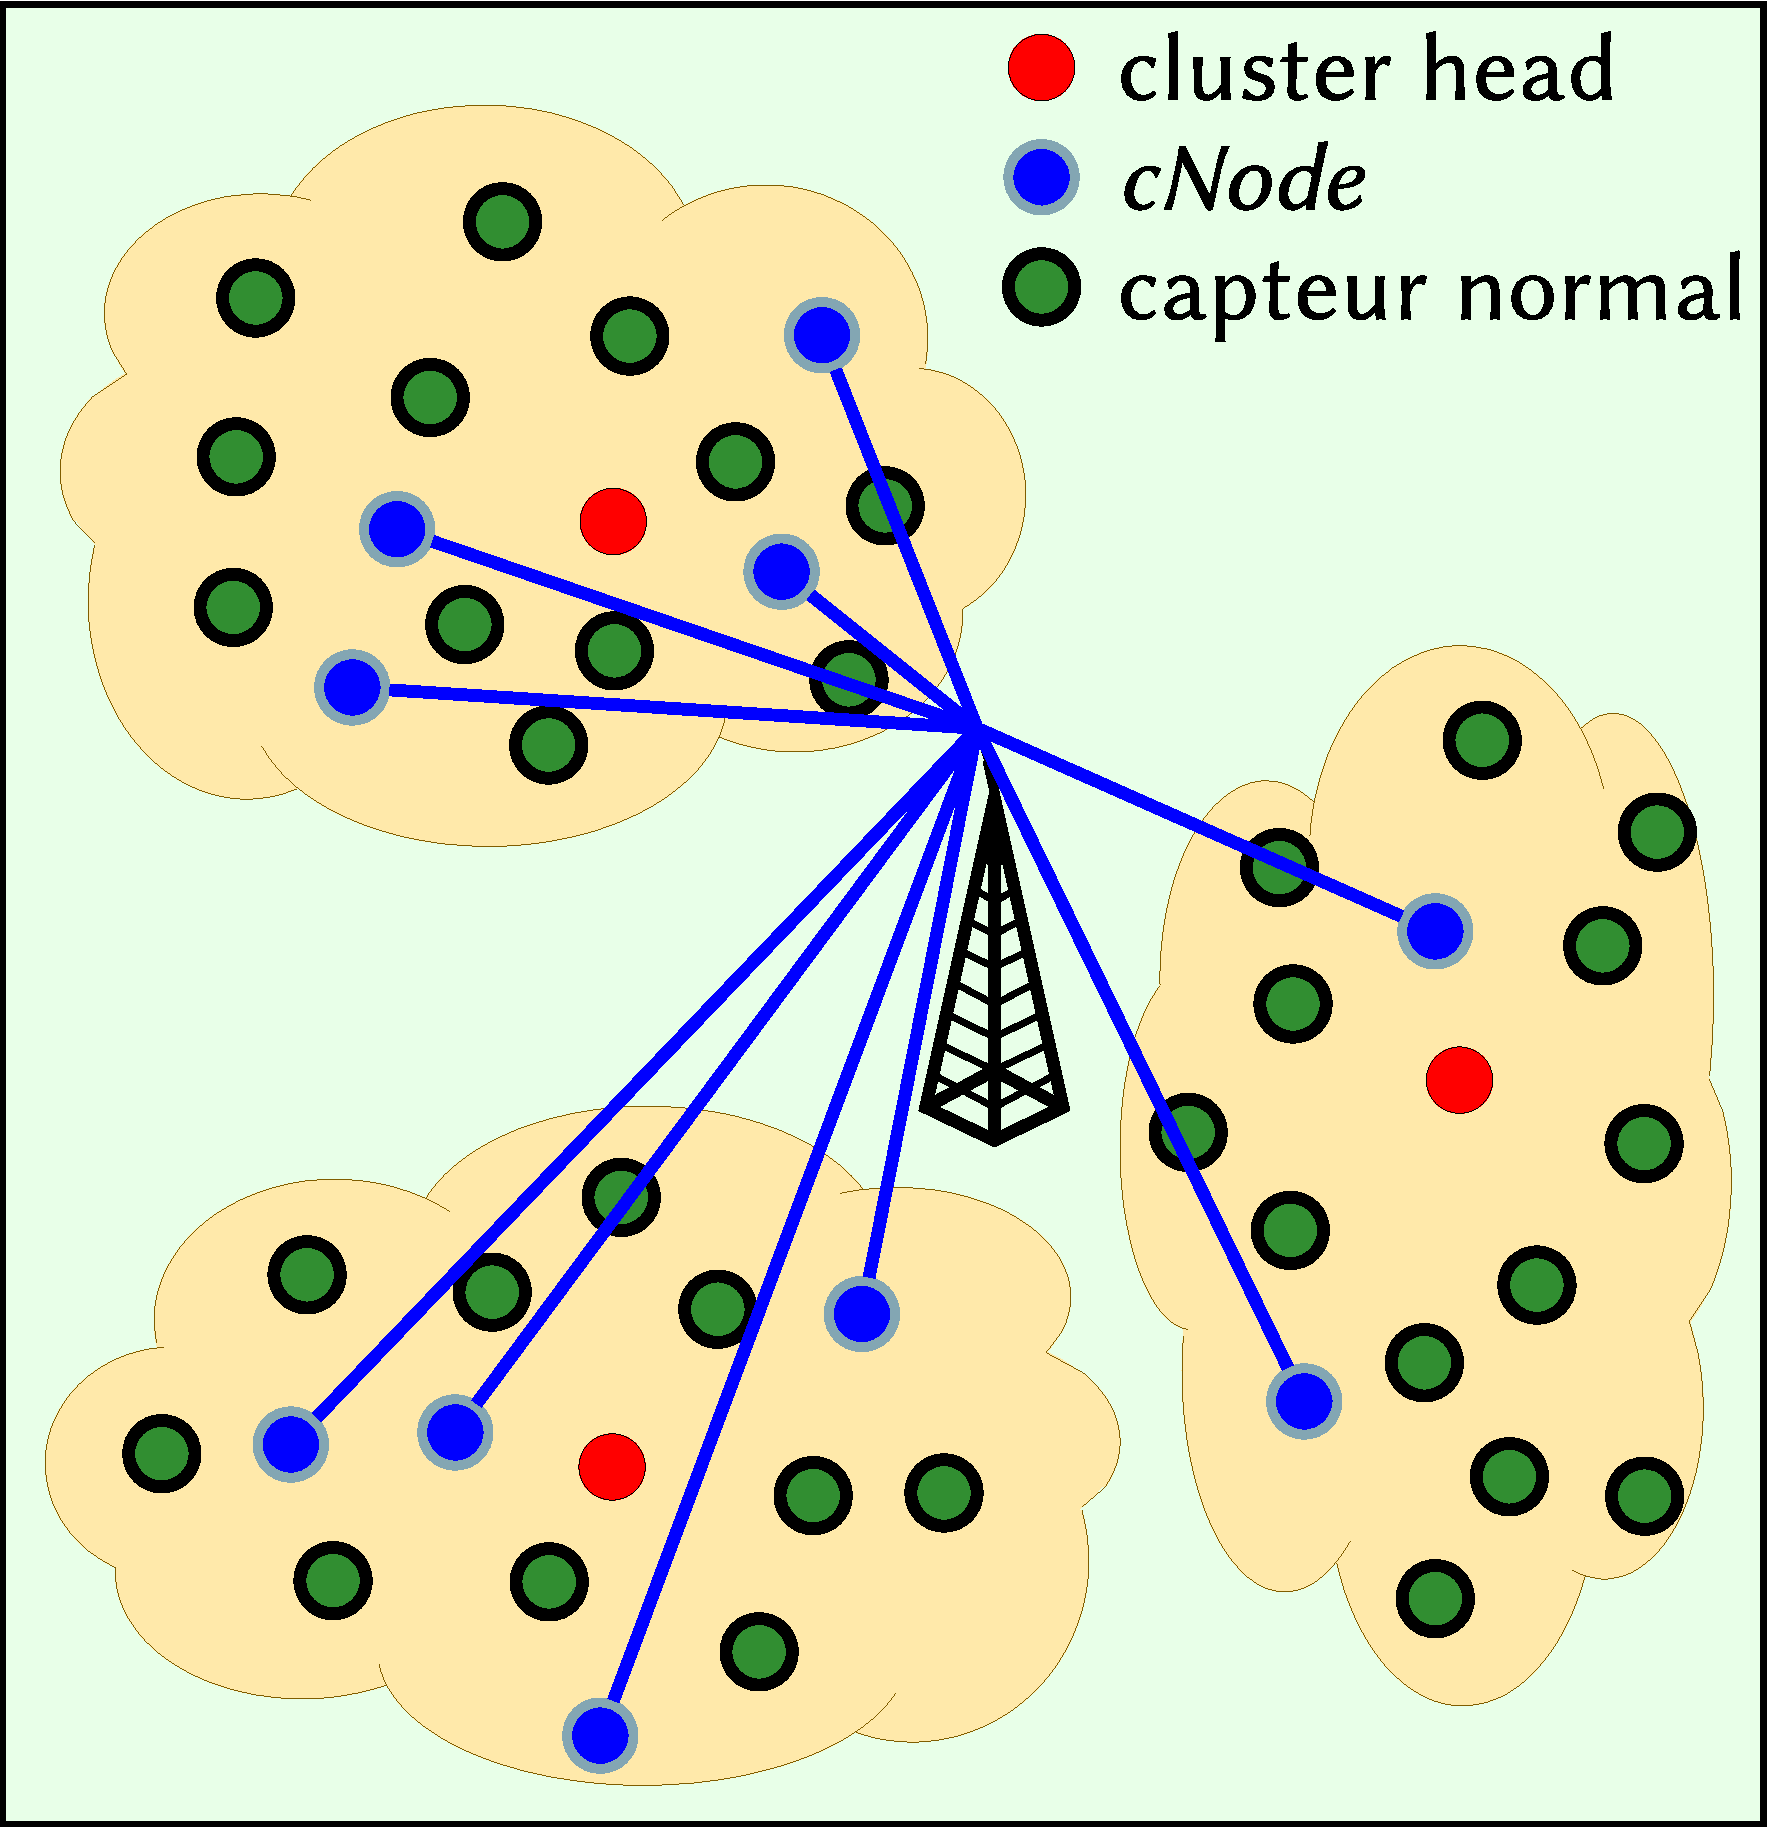
\includegraphics[width=.5\linewidth]{\chapterfig/elec_bs.pdf}
    \caption{Élection\index{selection@sélection!election@élection} des \cns réalisée par la \sdb}\label{sa:fig:elecbs}
\end{figure}

En revanche cette méthode n'offre pas une meilleure fiabilité que la précédente.
Si un nœud compromis se déclare en temps que \CH, il risque fortement d'annoncer à la \sdb que son cluster est vide (il enverrait une liste vide en lieu et place de la liste des capteurs qui sont réellement présents dans son cluster).
Dans ce cas, la \sdb ne déclarera aucun \cn dans le cluster attaqué, et le \CH compromis ne sera pas détecté.
Pour parer à cette éventualité, la \sdb pourrait agir autrement lorsqu'elle reçoit une liste de capteurs vide.
Plus spécifiquement, elle devrait considérer que les nœuds dont elle n'a pas eu de nouvelles \via les listes des \CH ne sont peut-être pas simplement morts, mais escamotés par un \ch corrompu.
Ces nœuds disparus devraient donc être considérés comme potentiellement éligibles, de sorte que certains d'entre eux au moins soient déclarés \cns.

L'inconvénient majeur de cette méthode est le fait que la nature distribuée de l'\election (avec tous les avantages qu'apporte un algorithme distribué) est complètement
perdue.

Les avantages et inconvénients de chacune de ces trois méthodes présentées sont résumés dans la \tabref{sa:table:elec}.
\begin{table}[ht]
    \caption{Avantages et inconvénients de chaque méthode}\label{sa:table:elec}
    \medskip
    \begin{small}
        \tabulinesep=.5ex%
        \begin{tabu}{X[1,c,m] X[2,l,m] X[2,j,m]}
            \toprule
            \textsc{Méthode} & \textsc{Avantages} & \textsc{Inconvénients} \tabularnewline
            \midrule
            Auto-élection des \cns (selon le modèle de \leach)    & %
                \textbullet\;Très simple à mettre en œuvre\newline%
                \textbullet\;Pas d'envoi de paquets à travers le réseau pour désigner les \cns%
                & %
                \textbullet\;Chaque nœud doit calculer un nombre pseudo-aléatoire\newline%
                \textbullet\;Ne tient pas compte de la topologie du réseau\tabularnewline
            \midrule
            Élection des \cns par les \chs                        & %
                \textbullet\;Seuls les \CH calculent les nombres pseudo-aléatoires%
                & %
                \textbullet\;Si le \CH est compromis, il ne désigne aucun \cn (un nœud compromis peut se déclarer \CH à chaque ronde de \leach)\tabularnewline
            \midrule
            Élection des \cns par la \sdb                & %
                \textbullet\;Aucun calcul réalisé par les nœuds\newline%
                \textbullet\;Distribution spatiale idéale des \cns%
                & %
                \textbullet\;Si le \CH est compromis, il déclare un cluster vide\newline%
                \textbullet\;Perte de l'aspect décentralisé de l'algorithme\tabularnewline
            \bottomrule
        \end{tabu}\index{selection@sélection!auto-élection}\index{selection@sélection!election@élection}
    \end{small}
\end{table}
